\chapter{Opis rozwiązania}
\label{cha:Opis rozwiązania}

W poniższym rozdziale omówione zostaną kroki pracy.

\section{Transmisja danych}
\label{sec:transmisjaDanych}

Pierwszym aspektem który należy rozwiązać jest sposób przesyłania danych. Problem ten jest szczególnie istotny w omawianej pracy z uwagi na możliwość przesyłania informacji o granica lub innych liniach przezentowanych na mapie. Do opisu kwadratowego obszaru wymagane jest przesłanie informacji o 4 punktach. Jeżeli będziemy chcieli przekazać dokłądniejszy zarys obszaru, zaprezentować granicę państwa lub linię frotnu wojennego linia prosta w większości przypadków będzie zbyt ogólnym przybliżeniem, nie oddającym prawdziwej sytuacji.

Z raportu Akamai wynika że śrenia przepływność łączy internetowych dla użytkowników korzystających z puli adresów IP przeznaczonych dla Polski w I kwartale 2012 r. wynosiła 5Mb/s  \underline{\texttt{http://www.rp.pl/artykul/924483.html}} (dostęp 13.04.2014). Jest to bardzo dobry wynik któy plasuje Polskę w czołówce rankingu. Pomimo tego nie można pominąć faktu optymalizacji zapytać i danych przesyłanych, wymieniane dane pomiędzy użytkownikiem a serwerem powinny być jak najmniejsze. Duża popularność urządzeń mobilnych w których dostęp do internetu jest zapewniany często poprzez sieć bezprzewodową a dostęp do interentu nie jest jeszcze tak dogodny jak jest to w przypadku użytkowników stacjonarnych  wymusza optymalizację.

Kolejnym powodem dla którego odpowiedzi serwera powinny być jak najlżesze jest koszt pracy samego serwera. Jest to szczególnie widoczne w dużych aplikacjach mających wiele urzytkowników, czas jaki jest przeznaczany dla pojedyńczego użytkownika jest mnożony przez ich ilość. Z tego powodu zawsze podczas zwiększania ilości użtkowników korzystających z aplikacji następuje czas w którym należy zacząć korzystać z dodatkowego serwera. Celem programisty tworzącego kod który będzie wykorzystywał zasoby serwera(zarówno czas jak i pamięć) jest dbanie aby moment w którym niezbędne będzie korzystanie z większej ilośći maszym nastąpił przy jak największej ilości użytkowników.

xml - 729  557
json - 695  400


\section{Możliwości HTML5}
\label{sec:html5}

HyperText Markup Language,  hipertekstowy język znaczników
Pozwala na opisanie struktury informacji zawartych na stronie internetowej, to dzięki niemu przeglądarka moze rozróżnić takie elementy jak hiperłącze,akapit czy chociażby nagłówek.

Podobnie jak w przypadku XML, tak i tutaj wymagane jest aby wykorzystywane znaczniki umieszczane były w nawiasach ostrokątnych, a każdy z nich miał swoje domknięcie.

Poprawnym zapisem jest <p>Wiadomość<p> który oznacza pojedyńczy akapit. Zapis <p>Wiadomość<p>, który różni się od poprzedniego brakiem znaku "" w drugim znaczniku, czyni to ten zapis niepoprawnym. Istnieje możliwość aby wykorzystać pojedyńczy znacznik przykładem jest <br> określający nową linię która będzie widoczna na stronie.

Obecnie używany standart HTML4 ma niestety wiele ograniczeń, z tego powodu pracowano nad jego następnikiem. 22 stycznia 2008 W3C opublikował HTML5, wtedy jeszcze jako jedynie szkic.

Bardzo ciekawym i wartym zainteresowania dodanym elementem w nowej wersji jest obecność znaczniku canvas. Pozwala on na dynamiczne , skryptowe renderowanie kształtów i obrazów. Dzięki temu obiektowi możliwe stało się tworzenie animacji czy nawet gier działających w przeglądarce bez konieczności używania dodatkowych wtyczek czy programów.

\underline{\texttt{http://techtrendy.pl/title,Pierwsza-gra-3D-napisana-w-HTML5,wid,14102779,wiadomosc.html?ticaid=6107dc}}

Przykładem wielkich możliwości jakie dostarcza udoskonalony język jest fakt iż już w roku 2011 powstała pierwsza trójwymiarowa gra stworzona w całości przy użyciu HTML5. Przykład grafiki widoczny jest na rysunku \ref{fig:html3d}.
Wcześniej takie efekty możliwe były jednynie przy wykorzystaniu technologi Flash, jej wadą była drudność edycji gotowego produktu, wyganało to specjalnego oprogramowania. Fakt tworzenia pliku wykonywalnego którego nie było możliwości edycji wymuszał dostęp do kodów źródłowych, czyli plików które tworzył autor programu.

\begin{figure}[H]
  \centering
    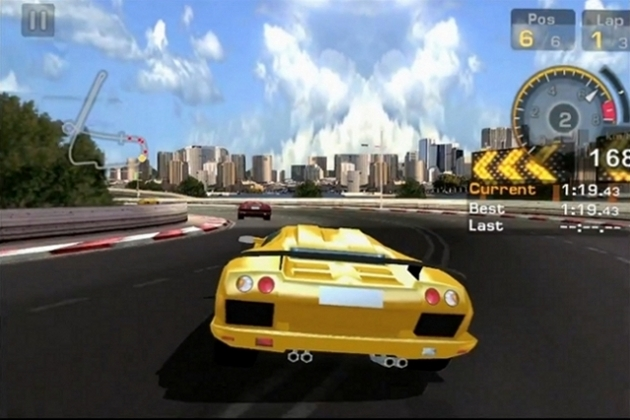
\includegraphics[width=100mm]{ge/html5_3d.jpg}
  \caption{Pierwsza gra 3D w html5.}
  \label{fig:html3d}
\end{figure}

Konkretną funkcjonalnością która wydaje się być przydatna w omawianym projekcie jest możliwość rysowania kształtów geomeycznych, również na innych obrazach. Przykładem wykorzystania tej technologi jest \ref{fig:canvas1} na którym przy pomocy okręgu zaznaczono rynek główny w Krakowie i jego okolice, możliwość zmiany przejżystości narysowanego kształtu pozwala aby obraz podnim był nadal widoczny.

  \begin{figure}[H]
  \centering
    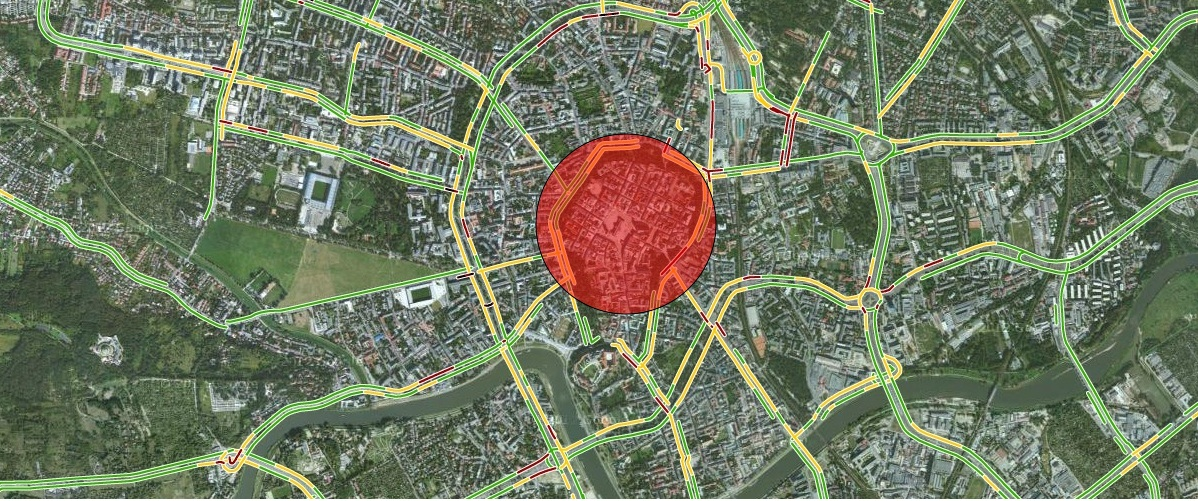
\includegraphics[width=100mm]{ge/canvas1.jpg}
  \caption{P.}
  \label{fig:canvas1}
\end{figure}

\lstset{language=JavaScript}
\begin{lstlisting}[caption=json]

      var canvas = document.getElementById('myCanvas');
      var context = canvas.getContext('2d');
      var imageObj = new Image();
	
      imageObj.onload = function() {
      context.drawImage(imageObj, 69, 50);
	  context.beginPath();
      context.arc(canvas.width / 2, canvas.height / 2, 90, 0, 2 * Math.PI, false);
      context.fillStyle = "rgba(255, 0, 0, 0.5)";
      context.fill();
      context.stroke();
      };
      imageObj.src = './gm_1.jpg';

\end{lstlisting}

\subsection{Wykorzystanie HTML5}
\label{subsec:htmluse}

Wstępne założenia zakładały wykorzystanie możliwości rysowania kształtów przy użyciu ogólnodostępnych map. Rozważania w sekcji \ref{sec:Rodzaje map} wskazały że najlepszym wyborem są Google Maps. Niestety opcja rysowania kształtów któa dostarcza HTML5 wymaga uzycia znacznika canvas, nie jest to kompatybilne z metodą wykorzystywania maps dostarczanych od omawianej firmy która wymaga wykorzystanie znacznika div.W momencie tworzenia tej pracy nie ma możliwości współpracy wybranych map z technologią rysowania kształtów geometrycznych. Sytuacja taka wymusza wykorzystanie innego rozwiązania do tworzenia interesujących nas warstw.

\subsection{Storage}
\label{subsec:storage5}
Inną ciekawą funkcją omówioną w podręczniku do HTML5  \cite{html5dive} jest Storage. Pozwala on na przechowywanie danych w przeglądarce użytkownika. Różnicą w stosunku do ciasteczek które również potrafią przechowywać informacje o konretnym użytkonwniku jest:
\begin{itemize}
\item
Większy rozmiar dostępnej pamięci m.in. Chrome 5MB \nocite{chrome5mb}, IE 10
\item
Informacje przechowywane są po stronie użytkownka, nie są przesyłane za każdym razem do serwera.
\item
Informacja może być przechowywana przez długi okres czasu.
\end{itemize}



Dodatkowo nie można pominąć faktu istnienia dwóch rodzaii tej pamięci.
\begin{itemize}

\item
Session Storage
Dane przechowywane są w kontekście sesji użytkownika, są one tracone w momencie zamknięcia okna przeglądarki.

\item
Local Storage
Teoretycznie dane są przechowywane w nieskończoność, do momentu kiedy użytkonwik nie usunie ich. Zamknięcię sesji nie powoduje czyszczenia danych.

\end{itemize}

Powodem który wymaga wykorzystania tego typu pamięci jest możliwość przechwowywania danych nad którymi użytkonwik pracuje w aktualnym czasie. Nie potrzebuje on informacji które były dla niego istotne podczas poprzedniej wizyty,sesji. Sytuacja ta jednoznacznie wskazuje że lepszym wyborem jest wybór pamięci sesyjnej(Session Storage).


Wadą tej pamięci jest jej interfejs. Obecnie przechowywany sposób danych to mapowanie w postaci napis->napis. Wymusza to aby każde dane które chcemy przechować muszą być w formie ciągu znaków. Przykład \ref{lis:storage} przedstawia w jaki sposób możemy obiekt zawierający imię i nazwisko zapisać w pamięci. Linia 4 przedstawia obiekt w postaci któej chcielibyśmy go przechować. Niestety zwykłe przypisanie do zmiennej w pamięci powoduje że jedynie typ instancji zostaje zapisany. Aby móc zapisać w poprawnej formie dane musimy doknać serializacji danych. Czynność tą możemy wykonać przy pomocy metody stringify z obiektu JSON, wynikiem jest ciąg znaków który możemy bez problemu zapisać w pamięci sesyjnej. Do odzyskania pierwotnego obiektu, odtworzenia go z zapisanego napisu wykorzystujemy metodę parse również z obiektu JSON.

\lstset{language=JavaScript}
\label{lis:storage}
\begin{lstlisting}[caption=json]
      uzytkownik={};
      uzytkonwik.imie='Jan'
      uzytkownik.nazwisko='Kowalski'
      //uzytkownik : Object {imie: "Jan", nazwisko: "Kowalski"}
      
      sessionStorage.u1 = uzytkownik
      //sessionStorage.u1 : "[object Object]"
      
      sessionStorage.u2 = JSON.stringify(uzytkownik)
      //sessionStorage.u2 : "{"imie":"Jan","nazwisko":"Kowalski"}"
      
      uzytkonwik2 = JSON.parse(sessionStorage.u2)
      //uzytkonwik2 : Object {imie: "Jan", nazwisko: "Kowalski"}
\end{lstlisting}



Wsparcie dla pamięci Storage nie jest obecne zazwyczaj w nowszych wersach przeglądarek. Na stronie \underline{\texttt{http://www.html5rocks.com/en/features/storage}} możemy sprawdzić aktualny stan większości przęglądarek.

\subsection{Web SQL Database}
\label{subsec:websql}

Koljenym ciekawym rozwiązaniem problemu przechowywania danych po stronie klienta jest Web Sql Database. 
Jest to baza danych która została umieszczona po stronie klienta. Jest to dodatkowa warstwa która korzysta z SQlite.
Zaletą takiego rozwiązania jest przeżucenie kosztów obliczeniowych na stronę klienta,operacje takie jak sortowanie, filtrowanie na bazie danych wykonywane są przy wykorzystaniu zasobów komuptera klienta.

Nie wątpliwą zaletą w stosunku do omówionej w rozdziale \ref{subsec:storage5} pamięci jest możliwość ustalenia wielkości zalokowanej wielkości pamięci. Dzięki temu nie jesteśmy ograniczenie granicą maksymalnie 5MB w więkoszości przeglądarek. 

Przykład wykorzystania został zaprezentowany na przykładzie. Po stworzeniu bazy danych o nazwie ExampleDataBase i rozmiarze 2MB możemy korzystać z niej jak z każdej innej bazy danych. Możliwe są m.in. operacje tworzenia table(linie 3-5), wstawiania danych(parametry podajemy po treści zapytania, następnie możemy podać funkcje które zostaną wykonane w momencie sukcesu lub w przypadku wystąpienia błędu). Odczyt danych (linie 13-18) jest analogiczny do pozostałych operacji, dodatkowo pokazano w jaki sposób możliwa jest iteracja po otrzymanych wynikach.

Wadą tego rozwiązania jest jego popularność.Na stronie browser stats  możemy sprawdzić jaka jest aktualnie popularność poszczególnych przeglądarek na świecie. Porównując te dane z dostępnością Web Sql dostępną na stronie \underline{\texttt{http://www.html5rocks.com/en/features/storage}} (dostęp) możemy wnioskować że prawie 45\% użytkowników( korzystających z IE i Firefox) nie mogą korzystać z tego rozwiązania. Fakt ten dyskfalfikuje je.

\lstset{language=JavaScript}
\label{lis:webSql}
\begin{lstlisting}[caption=json]
      var db = window.openDatabase("ExampleDataBase", "1.0", "Description", 2 * 1024 * 1024);
      
      db.transaction(function(tx) {
        tx.executeSql("CREATE TABLE TableTest (id REAL UNIQUE, text TEXT)");
      });
      
      db.transaction(function(tx) {
        tx.executeSql("INSERT INTO TableTest (id, text) VALUES (?, ?)", [1, 'test'],
        onSuccess,
        onError);
                });
                
      db.transaction(function(tx) {
        tx.executeSql("SELECT * FROM TableTest", [], function(tx, result) {
            for (var i = 0, item = null; i < result.rows.length; i++) {
                ...
			}
        });
      });
\end{lstlisting}

\subsection{IndexedDB}
\label{subsec:indexDB}

Trzecim rozwiązaniem jest indexDb.

\section{Oś czasu}
\label{sec:timeLine}

Tematem pracy oprócz wykorzystania i prezentacji danych na bazie informacji geograficznych jest ich połączenie z osią czasu, która pozwoliłaby na zmianę prezentowanych danych ze względu na interesujący nas okres czasu.

Ponieważ własna implementacja osi czasu która nieograniczałaby użytkownika, pozwala mu w pełni korzystać z możliwości pełnej aplikacji, która tylko w części składa się z możliwości manipulacji czasem postanowiono wykorzystać istniejące rozwiązanie.

Przeprowadzając badania rozwiązań głównymi aspektami na które zwrócono uwagę było:

\begin{itemize}

\item

Typ licencji
Niezwykle ważne jest aby końcowy projekt był całkowicie otwarty dla dalszego rozwoju, pozwalał użytkownikom na adaptację rozwiązań dla swoich potrzeb. Z uwagi na to licencja musi pozwalać na nieograniczoną modyfikację kodu źródłowego.

\item

Wykorzystywane technologie
Pamiętając że efektem końcowym powinien być framework odpowiadający szerokiemu gronowi odbiorców, będący jednocześnie darmowym ważne aby języki programowania wykorzystane przy jego tworzeniu też taki były. Oznacza to nie korzystanie z płatnych, wymagających licencji oprogramowań. Używane standarty powinny być rozpropagowane i używane przez szerokie grono obiorców.

\end{itemize}

Po długich i wnikliwych poszukiwaniach zdecydowano skorzystać z widget-u o nazwie Timeline który został stworzony przej projekt SIMILE działający na uczelni MIT. Pozwala on na bardzo dużą konfigurowalność dzięki czemu jego modyfikacja, nawet bez ingerencji w kod źródłowy jest bardzo prosta.
Projekt jest w stanie stworzyć kilka pasm któe będą określały interwały czasu. Pozwala to aby wynik końcowy był przejżysty bez względu czy prezentujemy wydarzenia które miały miejsce w okresie kilku minut czy setek lat.

Problemem który pojawił się było połączenie wybranego sposobu prezentacji osi czasu z mapą i elementami które powinny zmieniać się wraz z upływem czasu.

Rysunek \ref{fig:tm1} prezentuje możliwości tego projektu. Pasmo odpowiadają zakresom czasu, nie muszą on jednak być jednakowe w każdym miejscu. W zaprezentowanym przykładie dzień 23 listpoada uznany został za warty dokładniejszemu przyjżeniu,łatwo możemy z dokładnością co do godziny zmieniać zakres czasu.Natomiast kolejny miesiąc może być o wiele mniej ciekawy, a obszar przeznaczony dla niego być mniejszy niż ten posiadany przez wymieniony powyżej dzień.

Dla porównania \ref{fig:tm2} prezentuje o wiele prostszą konfigurację w której dolne pasmo podzielone jest przez miesiące, natomiast góre przez tygodnie.

  \begin{figure}[H]
  \centering
    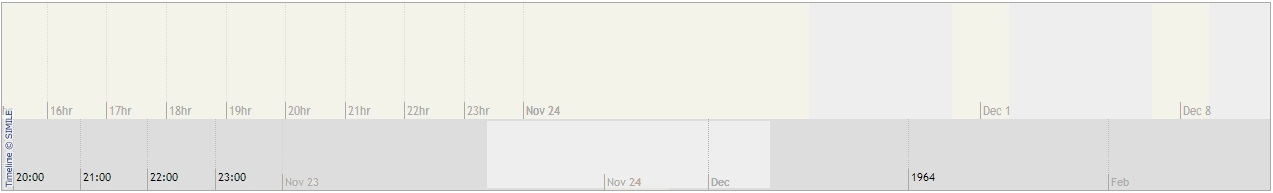
\includegraphics[width=150mm]{ge/tm1.jpg}
  \caption{Timeline}
  \label{fig:tm1}
\end{figure}

  \begin{figure}[H]
  \centering
    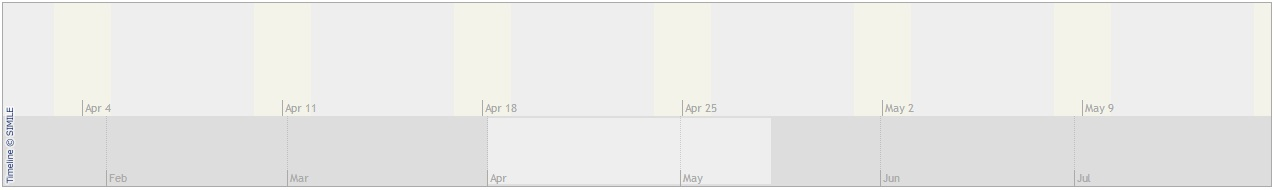
\includegraphics[width=150mm]{ge/tm2.jpg}
  \caption{Timeline 2}
  \label{fig:tm2}
\end{figure}
\section{Przybliżanie wyników}
\label{sec:przyblizanie}

Zmniejszanie ilości makretów w zależności od stopnia przyblizenia


\section{Parser kml}
\label{sec:scaner}



Format KML jest używany do reprezentacji danych graficznych w aplikacjach firmy Google, takich jak Google Maps czy Google Earth. Oparty jest na standardzie XML, wrażliwy na wielkość liter, wymusza ścisłą poprawność danych z formatem. Oznacza to że każdy tag, element ma ścisle określone miejsce i nie może pojawić się nigdzie indziej.


Aby tworzona aplikacja miała możliwość współpracy ze stworzonymi wczesniej zbiorami danych, mapami mimo faktu iż informacje te nie będą w pełni wykorzystywały możliwości frameworku, stworzony został parser plików kml. Dzięki temu możliwy jest import danych, uzupełnienie ich o dodatkowe informacje i zapis do własnego formatu.






\section{Interferjs}
\label{sec:Interferjs}


